\chapter{Resultados}
\label{chap:resultados}

\drop{E}{n} este capitulo se detalla el proceso y los pasos dados para la realización del 
proyecto. Se ha divido este apartado en dos partes puesto que realmente se 
desarrollaron dos proyectos, uno dependiente de los resultado del otro. 

\section{Análisis y viabilidad de las tecnologías}

Antes de desarrollar la aplicación final, la organización quería que se desarrollara una 
aplicación de pruebas que utilizará datos falsos y que se simularan las llamadas a las APIs. Con 
esto se quería comprobar el rendimiento de una aplicación con React Native, la fluidez, las 
transiciones entre pantallas, las animaciones y probar las posibles librerías que se 
podrían utilizar en la versión final.

\subsection{Sprint 0}

En esta primera fase se instalaron todas las herramientas necesarias para llevar acabo el 
proyecto. Se crearon los repositorios, uno en GitLab para la aplicación que se iba 
a crear y otro en GitHub para alojar el código fuente de la memoria. También se 
preparó Travis para que generara el pdf del anteproyecto y la memoria.

Después se creó un proyecto de React Native y se configuró en entorno y  las librerías 
necesarias como redux.

En la figura~\ref{fig:estructura} se puede apreciar la estructurad e carpeta del proyecto, la 
única variación se produjo en el Sprint 3 al eliminar la libreria Expo, que elimino la carpeta
.expo y generó dos carpetas nuevas: android e ios.

\begin{figure}[!h]
	\begin{center}
		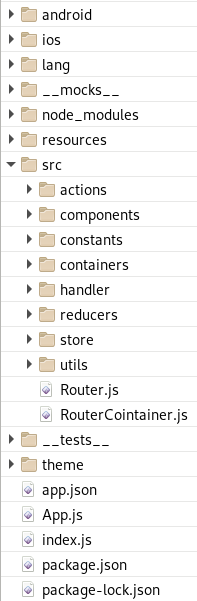
\includegraphics[width=0.2\textwidth]{./img/resultados/estructura.png}
		\caption{Estructura de directorios}
		\label{fig:estructura}
	\end{center}
\end{figure}

\subsection{Sprint 1}

En este primer Sprint se realizó la pantalla de bienvenida y otra para el inicio de sesión junto 
con la funcionalidad para iniciar sesión a través de la API de Nextinit en un entorno de 
pruebas y las animaciones requeridas.

También se creo otra pantalla que permite al usuario una vez ha iniciado sesión,
elegir en cuál de los Nextinit de los que dispone quiere entrar.

Además se preparó la navegación a través de la aplicación y se realizaron diversos 
cambios estéticos.

Se creó la pantalla inicial, a la que entra el usuario después de iniciar sesión y elegir el 
Nextinit. En esta pantalla se muestra una lista con todas las ideas con un scroll infinito
y un carrusel con los desafíos del Nextinit.

Se añadió una serie de pantallas que se muestran la primera vez que se inicia sesión 
en el Nextinit, son la pantalla con información de la RGPD, otra con el texto legal y 
un pequeño tutorial de la aplicación.

Se ha creado un menú lateral que permite acceder a las distintas secciones de la 
aplicación.

Se creó una pantalla a la que se accede desde un botón en la pantalla inicial,
en la que hay dos pestañas, una para ver las notificaciones del usuario y otra para
ver la actividad del Nextinit.


\subsection{Sprint 2}

En este Sprint se creo la pantalla que muestra la información de la idea seleccionada. Se creó 
una nueva pantalla accesible desde el menú lateral que muestra una lista con todas las ideas 
del usuario en las que se indica cuales están publicadas y las que son borradores. 

También se realizó la pantalla con un formulario para crear una nueva idea y una vista previa 
de la idea, en la que se muestra la misma pantalla que cuando se selecciona una idea pero con 
los datos recién introducidos.

Desde la vista previa de la idea se puede volver a la pantalla de edición de la idea o publicarla. En 
caso de publicarla, se da la posibilidad al usuario de realizar la primera inversión.

Al ver la información de la idea, si está buscando fondo aparece un botón que permite al usuario 
acceder al formulario para invertir en esa idea.

Se creó una pantalla accesible desde el menú lateral que muestra una lista con todos los desafíos 
disponibles

Se creó otra pantalla también accesible desde el menú lateral que muestra 4 pestañas en las que se 
pueden ver los rankings de usuarios que más dinero han invertido, que en más ideas han invertido, 
que más ideas han publicado y que tienen más dinero.

Se realizaron diversas pruebas para comprobar el desempeño de la aplicación en diversos idiomas como 
el francés, el chino y el ruso.

Se diseño una pantalla anterior a la de inicio de sesión con varias animaciones con el logo de Nextinit.

\section{Desarrollo de la aplicación}

\subsection{Sprint 0}

En este sprint se creó un nuevo proyecto, con algunas variaciones sustanciales en las librerías a 
utilizar y la estructura de carpetas. En este nuevo proyecto los sprints duraban 2 semanas. 

El primer 
días se celebró una reunión para presentar al equipo y conocer aspectos muy básicos del proyecto. Una 
vez presentado el equipo se expuso que rol desempeñaría cada uno dentro del equipo y se decidieron 
algunos aspectos sobre la gestión del proyectos, como por ejemplo la duración de los sprint.

Uno de objetivos de este sprint fue la formación del equipo, aprender o mejorar los conocimientos de 
React Navite y Javascript y también el de las librerías mas complejas que se iban a usar.

El objetivo al final del sprint era tener un equipo de desarrolladores formado y una aplicación 
con todo lo necesario para ser 
capaz de iniciar sesión en nextinit con un usuario y contraseña del sistema en Android o IOS.

Se cumplieron los objetivos del desarrollo pero no los formativos, varias personas del equipo estaban 
en otros proyectos y no pudieron dedicar el tiempo esperado por lo que la formación no fue tan completa 
como se planificó.

\subsection{Sprint 1}

Los objetivos de este sprint era hacer mejorar el inicio de sesión para que pudiera comprobar los credenciales de los
usuarios en el servidor de autenticación de los empleados de Viesgo que funcionaba con~\acf{ADFS}de Microsoft.

Se intentó validar unos credenciales de prueba siguiendo diversos manuales de Microsoft, además de 
diversas librerías que facilitaban la autenticación en React Native. Finalmente, no se pudo hacer funcionar
 este inicio de sesión puesto que el servicio de autenticación de Viesgo presentaba serios problemas de
 estabilidad y funcionamiento. Por lo que se tomó la decisión, de no incluir este inicio de sesión en las 
 primeras versiones hasta que Viesgo solventara sus problemas, algo que tardaría varios meses.

Al no poder realizar el inicio de sesión con los usuarios de Viesgo, se centraron los esfuerzos en realizar
la autenticación con los servidores de nextinit y conseguir que un usuario pudiera iniciar sesión con su 
usuario y contraseña y seleccionar el nextinit al que quería entrar de entre los que tuviera el usuario.

\subsection{Sprint 2}

Se crearon el inicio con la lista de ideas y el menú de la barra lateral
Durante el segundo Sprint se realizó la pantalla principal, en la que mostraba una lista de tarjetas con la 
información básica de las ideas publicadas en el Nextinit. En esta lista se mostraban las ideas públicas y 
en caso de ser un administrador, también las privadas.

También se realizó el sistema de navegación de la aplicación utilizando la librería React Navigation, que permite gestionar 
la navegación disparando acciones al igual que funcionaba el resto de la aplicación con redux. Se realizaron dos 
pilas de navegación independientes(ver Listado~\ref{code:navigation}), una con las pantallas de la aplicación cuando el usuario no ha iniciado 
sesión y otra pila con las pantalla una vez iniciada sesión(ver Listado~\ref{code:login}). A su vez se creaba una nueva pila por cada grupo de pantallas(ver Listado~\ref{code:home}),
que entre otras cosas facilitaba la navegación entre ellas.

\lstinputlisting[float=ht, language=Javascript, caption = {Stack principal de navegación}, label = code:navigation ]{code/navigation.js}
\lstinputlisting[float=ht, language=Javascript, caption = {Stack con las sesión iniciada}, label = code:login ]{code/login.js}
\lstinputlisting[float=ht, language=Javascript, caption = {Stack principal, para la gestión de ideas}, label = code:home ]{code/home.js}

La mayor dificultad de este Sprint fue como en la mayoría, adaptarse al diseño dado por el diseñador. Hubo grandes problemas
para usar una imagen de fondo en toda la aplicación, incluida en la cabecera y que fueran totalmente transparente.

\subsection{Sprint 3}

Se creó una pantalla para ver los detalles principales de la idea seleccionada, en el siguiente sprint se añadiría el resto de pantallas 
para ver los demás detalles de la idea.

Durante este sprint se utilizó el desarrollo de la página de inicio para crear un componente que mostra una serie de ideas dadas. Se 
realizó con este componente la pantalla de mis ideas, que mostraba todas las ideas publicadas por el usuario, las publicas, las privadas y
los borradores de ideas sin publicar.

Además se comenzó, algunas de las secciones son opcionales y solo se mostraran si están activadas en 
el nextinit, además algunos elementos como los objetivos son los introducidos por la organización. 

Para crear la idea es necesario seleccionar una imagen de la idea, que puede ser seleccionada desde la galería o realizada con la cámara 
del dispositivo.

No se pudo completar la creación de las ideas como estaba planificado, por lo que se concluyó en el sprint siguiente.

\subsection{Sprint 4}

En este sprint se añadieron dos nuevas pestañas a la pantalla de ver la idea. Una de ellas es para ver y escribir comentarios de la idea, 
en la que también se puede contestar a comentarios previos. Y la otra pantalla es para ver las personas involucradas en la idea, entre 
las que se encuentran iversores, creadores de la idea, colaboradores que se han ofrecido ayudar para llevar a cabo la idea y el equipo 
que llevará a cabo el piloto de la idea.

Se terminó la creación de la idea, una vez creada ésta se guardaba como borrador. Posteriormente se mostraba una vista previa de 
como se vería la idea una vez publicada.

También se desarrollo la pantalla,anteriormente mencionada, que muestra la vista previa de la idea. Se refactorizó el código creado 
para la pantalla principal de ver idea, y se creó un componente reutilizable para la pestaña principal de ver idea y para la vista previa. En 
esta vista previa solo se muestran los detalles principales de la idea, no se muestra ni las personas involucradas en la idea ni los 
comentarios.

La mayor complejidad de este sprint fue el desarrollo de un carrusel que muestra los desafíos en la pantalla principal. El carrusel muestra una imágen del desafío, 
el título y las ideas que creadas para él.

\subsection{Sprint 5}

En este último sprint se trabajó principalmente en perfeccionar la aplicación y pulir pequeñas imperfecciones estéticas. 

Además utilizando el componente anteriormente refactorizado se creó la pantalla de ver desafío, con dos pestañas. Una con dicho compenente 
para mostrar la información principal del desafío. Y otra usando el componente anteriormente creado que mostraba una lista de ideas, para 
mostrar una lista de las ideas del desafío.

También se creó una pantalla de notificaciones con tres pestañas. En una de ellas de mostraba las notificaciones del usuario, si se ha invertido en una idea suya, si se la han comentado, si ha ganado dinero.. En otra de ellas se mostraba toda la actividad del 
nextinit, si se ha publicado nuevas ideas, si alguien ha comentado, etc. Y en la restante se muestra la información de las pestañas 
antesriores junta.

Por último, se creó una pantalla que muestra un perfil básico de usuario. Con una pestaña en la que se puede observar algúnas estaditicas básicas del usuario y con otra pestaña en la que se puede ver la actidad del usuario en el nextinit.


% Local Variables:
%  coding: utf-8
%  mode: latex
%  mode: flyspell
%  ispell-local-dictionary: "castellano8"
% End:
